\documentclass[11pt]{article}

\usepackage{graphicx}
\usepackage{csquotes}
\usepackage{courier}
\setcounter{secnumdepth}{4}

\title{Corner Location Errors}
\author{Adam Yedidia, Vickie Ye, Katie Bouman}

\begin{document}
\maketitle

One important source of error in the edge camera idea is the \emph{corner location error}. When studying a movie of the projection plane, it's important to know where the corner of the wall is in order to make an accurate reconstruction. Corner location errors occur when the corner of the wall is erroneously chosen to be the wrong place. Corner location errors introduce systematic error into the scene's reconstruction.

The corner occluder can be chosen automatically (by minimizing the intensity variation along the ``rays'' emanating from the corner onto the projection plane) or manually (by clicking by hand on where the corner is in the image). Both of these methods have the potential to introduce a corner location error.

\section{Edge Camera}

Exactly how bad are corner location errors? To answer this question, we consider the situation shown in Fig.~\ref{fig:corner}. Imagine a dark scene with a single bright object. We want to find the angular position of the bright object in the scene. We can do this by measuring $\theta$: the angle of the shadow it casts against the wall. When we find the angle at which the projection plane goes from light to dark, we will know what $\theta$ is.

This story is simple in the case when there is no corner location error. But what about the case where there is such an error?

\begin{figure}
\centering
\includegraphics[scale=0.6]{figs/corner.png}
\caption{This figure shows the setup for the toy problem of interest. The scene consists of a single bright object, whose angular position $\theta$ we want to learn. \label{fig:corner}}
\end{figure}

Fig.~\ref{fig:theta_sweep} shows this scenario. We can ``sweep'' the angle $\phi$ across the projection plane, and at the point where $\phi$ is midway between dark and light, we can presume that that is the object's angular position. When there is no corner location error, we will naturally get $\theta = \phi$, but when there is a corner location error, $\phi$ will depend on $\theta$ and other parameters in a more complicated way.

\begin{figure}
\centering
\includegraphics[scale=0.6]{figs/theta_sweep.png}
\caption{This figure shows the impact of a corner location error. In the error-free case, we would sweep $\phi$ across the projection plane (shown in green) hinging around the corner (the solid black line). But if made a corner location error, we would instead try to sweep $\phi$ across the projection plane erroneously (shown in blue) hinging around the false corner (shown with a dotted line). \label{fig:theta_sweep}}
\end{figure}


Fig.~\ref{fig:intensity_values} plots intensity against the sweeping angle $\phi$, both with and without a corner location error. Note that in the case where there is a corner location error, the maximum intensity value no longer takes on a maximum value of 1, but a value below 1. In the analysis that follows, we will call that value $l_{\mathrm{max}}$, and we will use $\l_{\mathrm{max}}/2$ as the ``transition point'' between light and dark. In other words, we will choose the $\phi$ that gives an intensity of $\l_{\mathrm{max}}/2$ as our estimate for $\theta$.

\begin{figure}
\centering
\includegraphics[scale=0.6]{figs/intensity_values.png}
\caption{This plot shows how the observed intensity values vary with $\phi$, in the case of correct corner location (in blue) and a corner location error ($(d_x, d_y) = (0.1, 0.2)$, in red). Note that in the case of a corner location error, the maximum value of the intensity does not reach 1. Note also that $d_x$ and $d_y$ are as a fraction of the radius of the projection plane, $r$, which here is taken to be 1. \label{fig:intensity_values}}
\end{figure}

Fig.~\ref{fig:greek} is a detailed illustration of the situation, showing the names for the variables that we'll use in our analysis. As the figure shows, we are presuming a corner location error of $(d_x, d_y)$ and a projection plane radius of $r$. We want to find what our estimate $\theta$, $\phi$, will be as a function of $\theta$ and in terms of $d_x, d_y$, and $r$.

\begin{figure}
\centering
\includegraphics[scale=0.5]{figs/greek.png}
\caption{This plot is intended as a reference for the meanings of each of the variables used in the calculations of $\phi$ as a function of $\theta$. \label{fig:greek}}
\end{figure}

Using Fig.~\ref{fig:greek} as a reference, we can make the following observations:

$$\beta = \tan^{-1}\left(\frac{d_x}{d_y}\right)$$
$$l_{\mathrm{max}} = r - d_y \tan(\theta) + d_x$$
$$f = r - \frac{l_{\mathrm{max}}}{2}$$
$$\alpha = \sin^{-1}\left(\frac{\sqrt{d_x^2+d_y^2}\sin(\theta-\beta)}{f}\right)$$
$$\gamma = \pi - \alpha - \theta + \beta$$
$$\phi = \pi - \gamma + \beta$$

This is how $\phi$ is expressed in terms of the parameters of the problem $(\theta, d_x, d_y, r)$.

What sort of error does this introduce? In order to study this question, we assumed that $d_x$ and $d_y$ were normally distributed with means of 0 and small (relative to $r^2$) variances $\sigma_x^2$ and $\sigma_y^2$. We generated many sample ($\theta$, $\phi$) pairs for each $\theta$ between 0 and $\pi/2$. We then measured the empirical means and variances of these pairs. Fig~\ref{fig:error_behavior} shows a few of our results.

\begin{figure}
\centering
\includegraphics[scale=0.6]{figs/error_behavior.png}
\caption{This plot shows the empirical mean (in blue) plus or minus one standard deviation (in red) of the error as a function of $\theta$. Here, $\sigma_x = 10^{-4}$ and $\sigma_y = 10^{-3}$. \label{fig:error_behavior}}
\end{figure}

Here were a few of our empirical findings:

\begin{enumerate}
    \item The mean error was always 0 for all values of $\theta, \sigma_x$ and $\sigma_y$.
    \item When $\sigma_x = \sigma_y$, the standard deviation of the error $\sigma_{\epsilon}$ was $2\sigma_x$ for all values of $\theta$.
    \item When $\sigma_x \not= \sigma_y$, the standard deviation of the error $\sigma_{\epsilon}$ varied between $2\sigma_x$ (for $\theta = 0$) and $2\sigma_y$ (for $\theta = \pi/2$).
\end{enumerate}

\section{Stereo Camera}

Another situation in which it makes sense to study corner location errors is in the case where there is a doorway just before the hidden scene, in which case we can use stereo vision to locate a moving object in two dimensions. What effect do corner location errors have on depth estimates, which are generally quite sensitive to noise? To be more precise, suppose that we call the axis along which the doorway lies the ``$x$-axis,'' and suppose we call the perpendicular axis (of depth into the room) the ``$z$-axis.'' Then, how much noise in the $z$ dimension will a corner location error cause?

To give an approximate sense of how much error results in the recovered $z$ position, we show the mean +/- one standard deviation in the $z$ dimension as a function of the true $x$-position of the object in Fig.~\ref{fig:depth_plots}

\begin{figure}
\centering
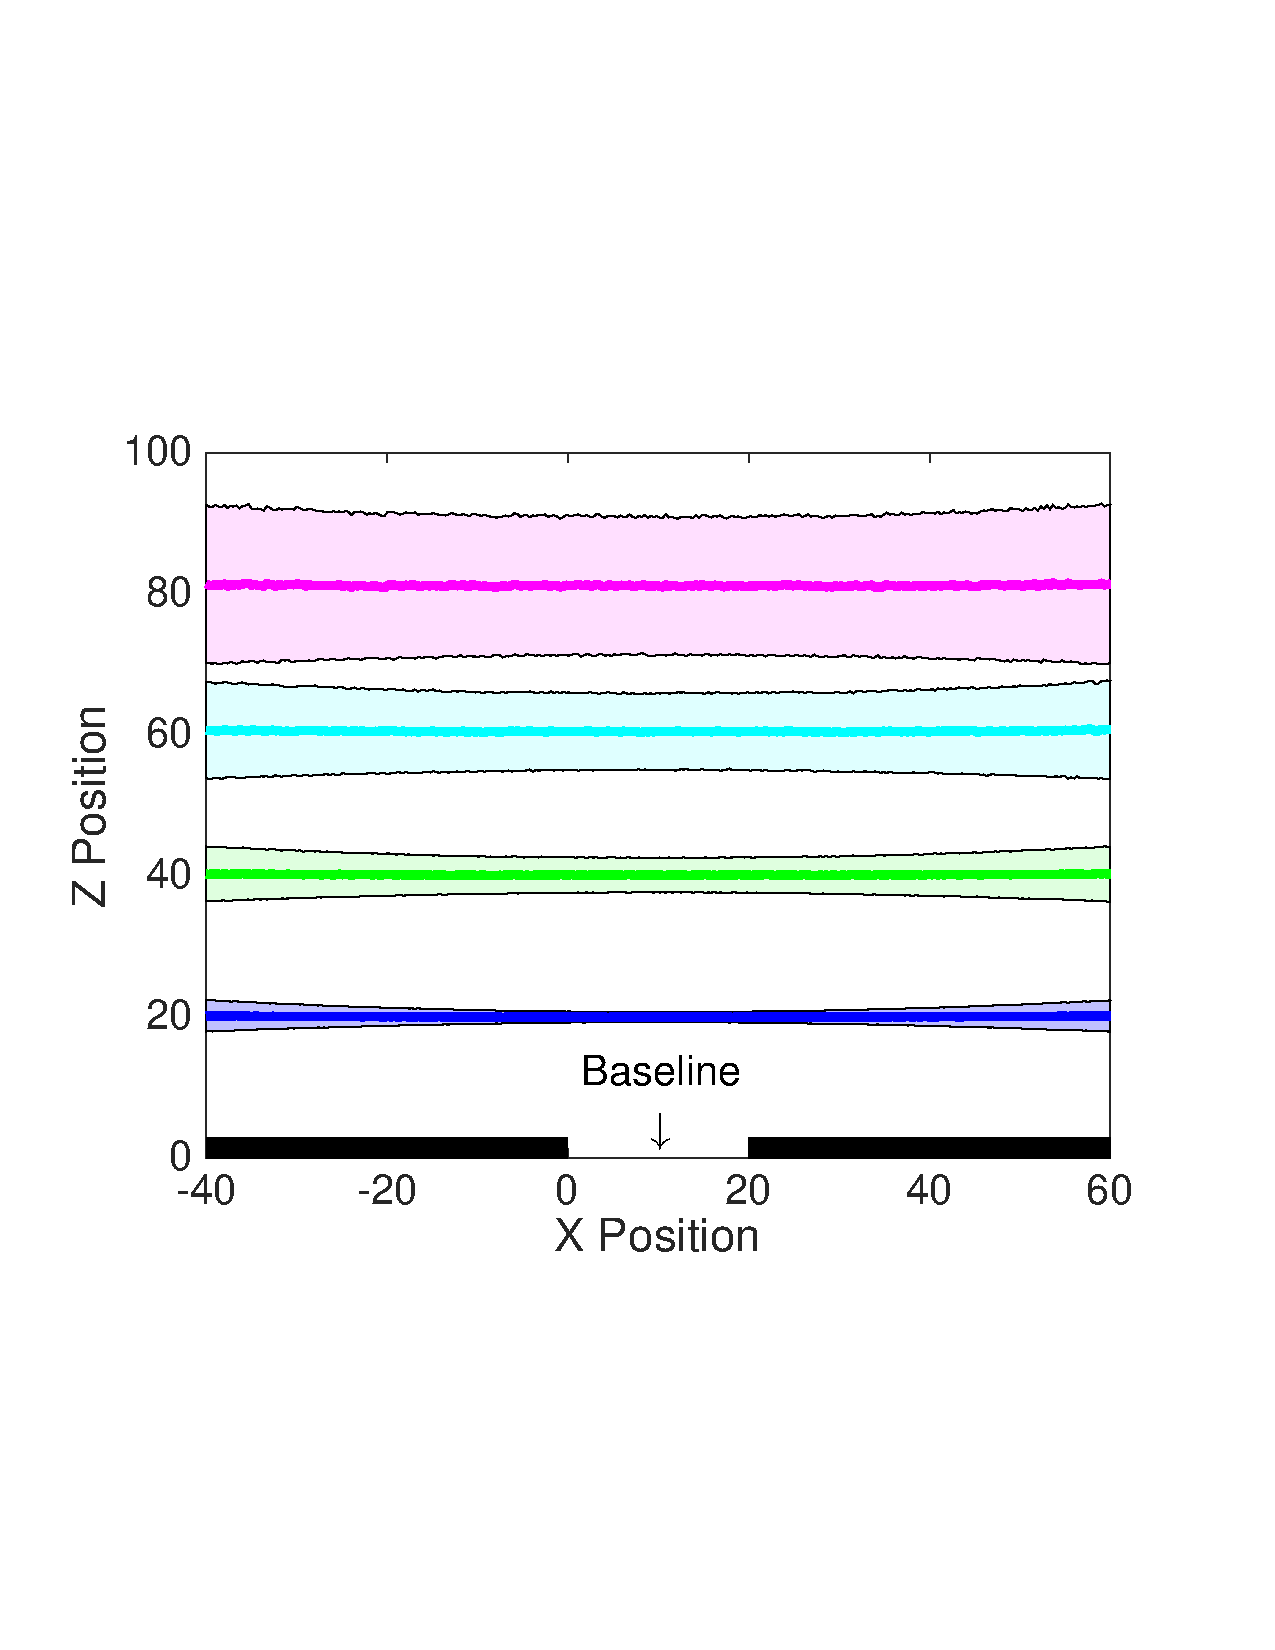
\includegraphics[width=0.7\linewidth]{figs/depth_plots.pdf}
\caption{The empirical means plus or minus one standard deviation of the estimated $P_z$ as a function of its $x$-coordinate, assuming true $P_z$ of 20, 40, 60, and 80. Here, the two corner location errors at each of the boundaries of the doorway are independent and subject to $\sigma_{\Delta x}^2 = \sigma_{\Delta z}^2 = 0.04$. We sample from a set of 1000 corner errors to approximate the mean and standard deviations empirically. \label{fig:depth_plots}}
\end{figure}

Note that the empirical means are centered at the true depths of the objects. This does \emph{not} mean that any single corner location error won't cause the depth of the reconstruction to be off systematically, only that on average, corner location errors that are normally distributed around the corners in question will push the reconstructed depths away as much as they pull them closer.

To see this systematic bias on its own, we can also study how a single corner error introduces systematic error in our reconstructions---after all, for a single experiment, we are likely to make a single corner error, and the resulting error in the depth calculations will extend across many $x$-coordinates as the subject of the experiment walks back and forth in the hidden scene. Figs.~\ref{fig:systematic_same} and~\ref{fig:systematic_diff} show the systematic bias for two distinct \emph{specific} corner location errors.

\begin{figure}
\centering
\includegraphics[width=0.7\linewidth]{figs/systematic_same.png}
\caption{The reconstructed depths of objects at depths 1, 2, 3, and 4, given a corner error of $\Delta y_1 = \Delta y_2 = 0.02$. \label{fig:systematic_same}}
\end{figure}

\begin{figure}
\centering
\includegraphics[width=0.7\linewidth]{figs/systematic_diff.png}
\caption{The reconstructed depths of objects at depths 1, 2, 3, and 4, given a corner error of $\Delta y_1 = -0.02$, $\Delta y_2 = 0.02$. Note that because of the different corner errors for each corner, there is the possibility of asymmetric behavior on either side of the doorway. \label{fig:systematic_diff}}
\end{figure}



\end{document}